\subsection{Ozone mixing ratios as function of NOx and Temperature} \label{ss:r_contours}

\begin{figure}%
    \centering%
    \caption{Contours of maximum ozone mixing ratio as a function of the total \ce{NO_x} emissions on the first day and temperature for each chemical mechanism and using both a temperature-dependent and -independent source of isoprene emissions.}
    \label{f:ozone_contours}%
    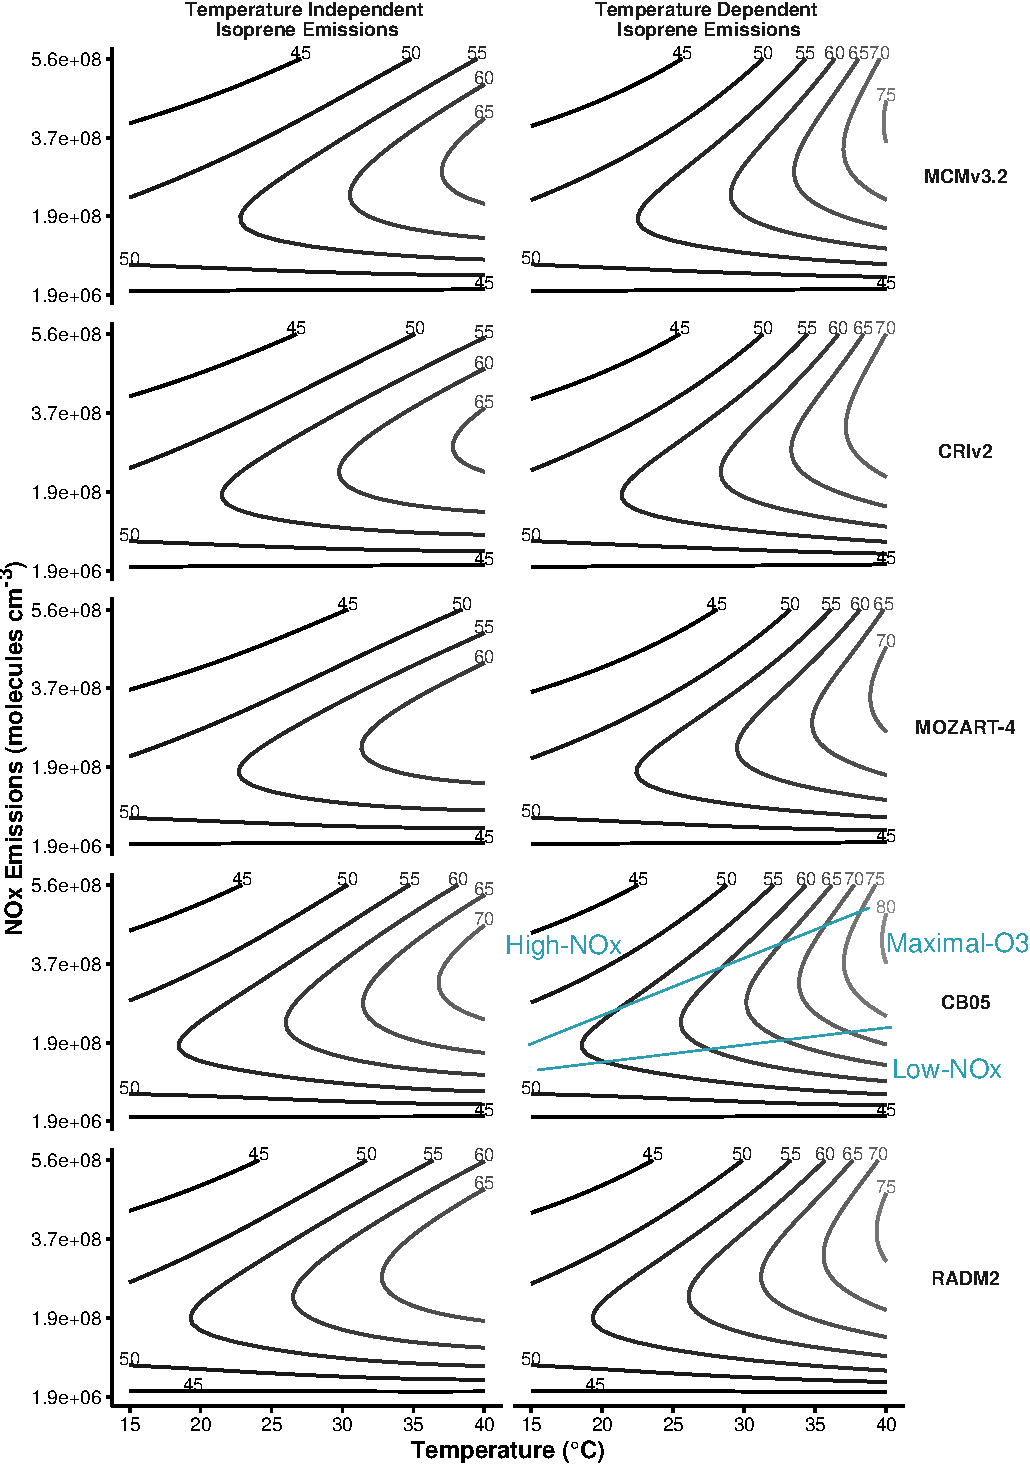
\includegraphics[width=\textwidth]{img/O3_comparison}
\end{figure}

\begin{figure}%
    \centering%
    \caption{Ozone mixing ratios at each temperature are allocated to different \ce{NO_x}-regimes of Fig.~\ref{f:ozone_contours}. The differences in ozone mixing ratios due to chemistry and emissions of Table~\ref{t:differences} are represented graphically for MOZART-4, the approach was used to calculate the differences with each chemical mechanism.}%
    \label{f:O3-T}%
    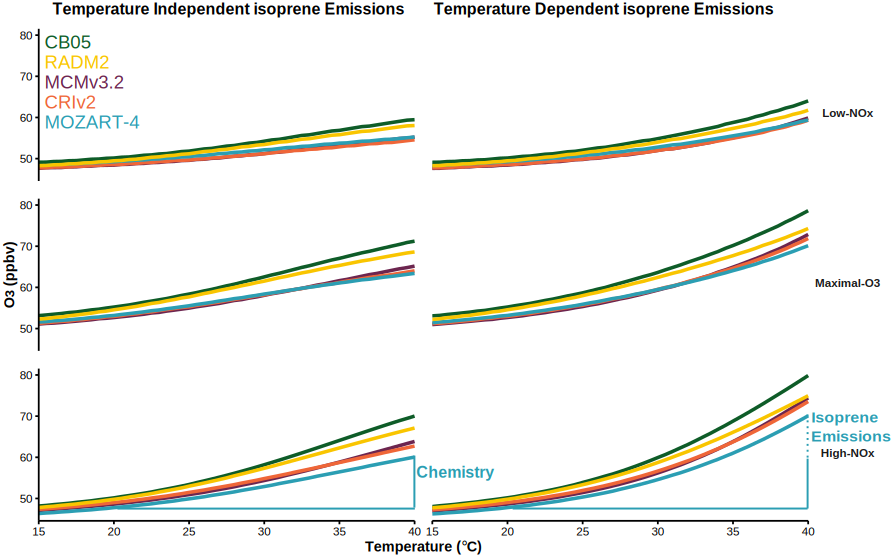
\includegraphics[width=\textwidth]{img/O3-T_correlation}%
\end{figure}

\begin{table}%
    \centering%
    \caption{Increase in ozone mixing ratio (ppbv) due to chemistry and emissions at $40$~$^{\circ}$C from reference temperature ($20$~$^{\circ}$C) in the \ce{NO_x}-regimes of Fig.~\ref{f:ozone_contours}.}%
    \label{t:differences}%
    \begin{tabularx}{\textwidth}{c|c *{3}{|c}} 
    \hline \hline
    \textbf{Chemical} & \textbf{Source of} & \multicolumn{3}{c}{\textbf{Increase in Ozone from 20~$^{\circ}$C to 40~$^{\circ}$C (ppbv)}} \\ \cline{3-5}
    \textbf{Mechanism} & \textbf{Difference} & \textbf{Low-\chem{NO_x}} & \textbf{Maximal-\chem{O_3}} & \textbf{High-\chem{NO_x}} \\ 
    \hline \hline
    \multirow{2}{*}{MCMv3.2} & Isoprene Emissions & 4.6 & 7.7 & 10.6 \\ 
    & Chemistry & 6.8 & 12.5 & 15.2 \\ \hline
    \multirow{2}{*}{CRIv2} & Isoprene Emissions & 4.8 & 7.9 & 10.8 \\
    & Chemistry & 6.0 & 11.1 & 13.7 \\ \hline
    \multirow{2}{*}{MOZART-4} & Isoprene Emissions & 4.1 & 6.7 & 10.0 \\
    & Chemistry & 6.0 & 10.2 & 12.3 \\ \hline
    \multirow{2}{*}{CB05} & Isoprene Emissions & 4.6 & 7.4 & 9.8 \\
    & Chemistry & 9.3 & 16.0 & 19.9 \\ \hline
    \multirow{2}{*}{RADM2} & Isoprene Emissions & 3.8 & 5.7 & 7.8 \\ 
    & Chemistry & 8.6 & 14.1 & 17.3 \\
    \hline \hline
\end{tabularx}

\end{table}

Figure~\ref{f:ozone_contours} depicts the maximum mixing ratio of ozone as a function of the total \ce{NO_x} emissions on the first day and temperature when using temperature-independent and temperature-dependent source of isoprene emissions for each chemical mechanism.
A non-linear relationship of ozone mixing ratios with \ce{NO_x} and temperature is reproduced by each chemical mechanism.

The highest mixing ratios of ozone in Fig.~\ref{f:ozone_contours} are produced at higher temperatures and high-\ce{NO_x} conditions, also ozone mixing ratios increase when using a temperature-dependent source of isoprene emissions.
Conversely, the least amount of ozone is produced with low-\ce{NO_x} conditions over the whole temperature range ($15$~--~$40~^{\circ}$C) when using both a temperature-independent and temperature-dependent source of isoprene emissions.

The non-linear relationship of ozone with \ce{NO_x} and temperature can be split into three \ce{NO_x}-regimes (low-\ce{NO_x}, maximal-\ce{O3} and high-\ce{NO_x}) based on the ratio of \ce{HNO3} to \ce{H2O2} used in \citet{Sillman:1995} to determine \ce{NO_x}-regimes for the non-linear relationship of ozone with \ce{NO_x} and VOC.
The low-\ce{NO_x} regime corresponds to the lower-left most area in Fig.~\ref{f:ozone_contours} where there is little increase in ozone with temperature, also called \ce{NO_x}-sensitive conditions.
The high-\ce{NO_x} regime is when ozone levels increase rapidly with temperature in Fig.~\ref{f:ozone_contours}, sometimes called \ce{NO_x}-saturated conditions.
Finally, the ridges of the contours in Fig.~\ref{f:ozone_contours} correspond to maximal-ozone production and we call this the maximal-\ce{O3} regime.
The ozone mixing ratios obtained in each simulation were assigned to a \ce{NO_x} regime based on the \ce{H2O2}:\ce{HNO3} of the simulation and Fig.~\ref{f:O3-T} illustrates the mean ozone mixing ratio at each temperature in these \ce{NO_x} regimes.

Calculating the difference in ozone mixing ratios at $40$~$^{\circ}$C from $20$~$^{\circ}$C when using a temperature-independent source of isoprene emissions gives the absolute increase in ozone due to faster chemistry.
When using a temperature-dependent source of isoprene emissions, the difference in ozone mixing ratios at $40$~$^{\circ}$C from $20$~$^{\circ}$C less the increase due to faster chemistry, gives the absolute increase in ozone due to increased isoprene emissions.
These differences are represented graphically in Fig.~\ref{f:O3-T} and summarised in Table~\ref{t:differences}.

Both Fig.~\ref{f:O3-T} and Table~\ref{t:differences} highlight that the absolute increase in ozone at $40$~$^{\circ}$C from $20$~$^{\circ}$C is largest with high-\ce{NO_x} conditions.
The increase in ozone mixing ratio at $40$~$^{\circ}$C from $20$~$^{\circ}$C due to faster chemistry with high-\ce{NO_x} conditions is almost double that with low-\ce{NO_x} conditions.
We shall explore which chemical processes are responsible for the increases in ozone mixing ratios at $40$~$^{\circ}$C from $20$~$^{\circ}$C by analysing \ce{O_x} production budgets in Sect.~\ref{ss:r_budgets}.

Comparing the response of ozone mixing ratios to temperature in the reduced chemical mechanisms (CRIv2, MOZART-4, CB05 and RADM2) to the near-explicit MCMv3.2 chemical mechanism shows that the largest differences from the MCMv3.2 occur in the maximal-\ce{O3} and high-\ce{NO_x} regimes.
Table~\ref{t:differences} also indicates that all reduced chemical mechanisms, except RADM2, have similar increases in ozone due to temperature-dependent isoprene emissions to MCMv3.2.
RADM2 produces $3$~ppbv less ozone than the MCMv3.2 due to temperature-dependent isoprene emissions consistently in each \ce{NO_x} regime, indicating that this difference is due to how isoprene degradation chemistry is treated in RADM2.

The Tagged Ozone Production Potential (TOPP) of isoprene is a measure of the number of molecules of ozone produced per molecule of isoprene emitted and \citet{Coates:2015} shows that less ozone is produced from isoprene degradation using RADM2 than with MCMv3.2.
The degradation of isoprene has been extensively studied and it is well-known that the species methyl vinyl ketone (MVK) and methacrolein are signatures of isoprene degradation.
All chemical mechanisms used in our study do explicitly include MVK and methacrolein (or in the case of CB05, a lumped species representing both these secondary degradation products) production during isoprene degradation except RADM2.
RADM2 does not include methacrolein and the ketone species included in RADM2 represents a mixture of acetone and methyl ethyl ketone (MEK), thus the secondary degradation of isoprene in RADM2 is unable to represent the ozone production from the further degradation of its signature degradation products MVK and methacrolein.
More recent versions of RADM2, RACM \citep{Stockwell:1997} and RACM2 \citep{Goliff:2013}, sequentially include methacrolein and MVK and with these updates the TOPP values of isoprene reported in \citet{Coates:2015} are similar to the TOPP value of isoprene in the MCMv3.2.

\subsection{Ozone budgets} \label{ss:r_budgets}

\begin{figure}%
    \centering%
    \caption{\ce{O_x} production budgets normalised by the total oxidation rate of emitted VOC in the \ce{NO_x}-regimes of Fig.~\ref{f:ozone_contours}. The budgets are allocated to the categories of inorganic reactions, peroxy nitrate (RO2NO2) decomposition, reactions of NO with HO2, non-acyl peroxy radicals (RO2) and acyl peroxy radicals (ARO2). All other reactions contributing to \ce{O_x} budgets are allocated to `Other Organic'.}%
    \label{f:ozone_budgets}%
    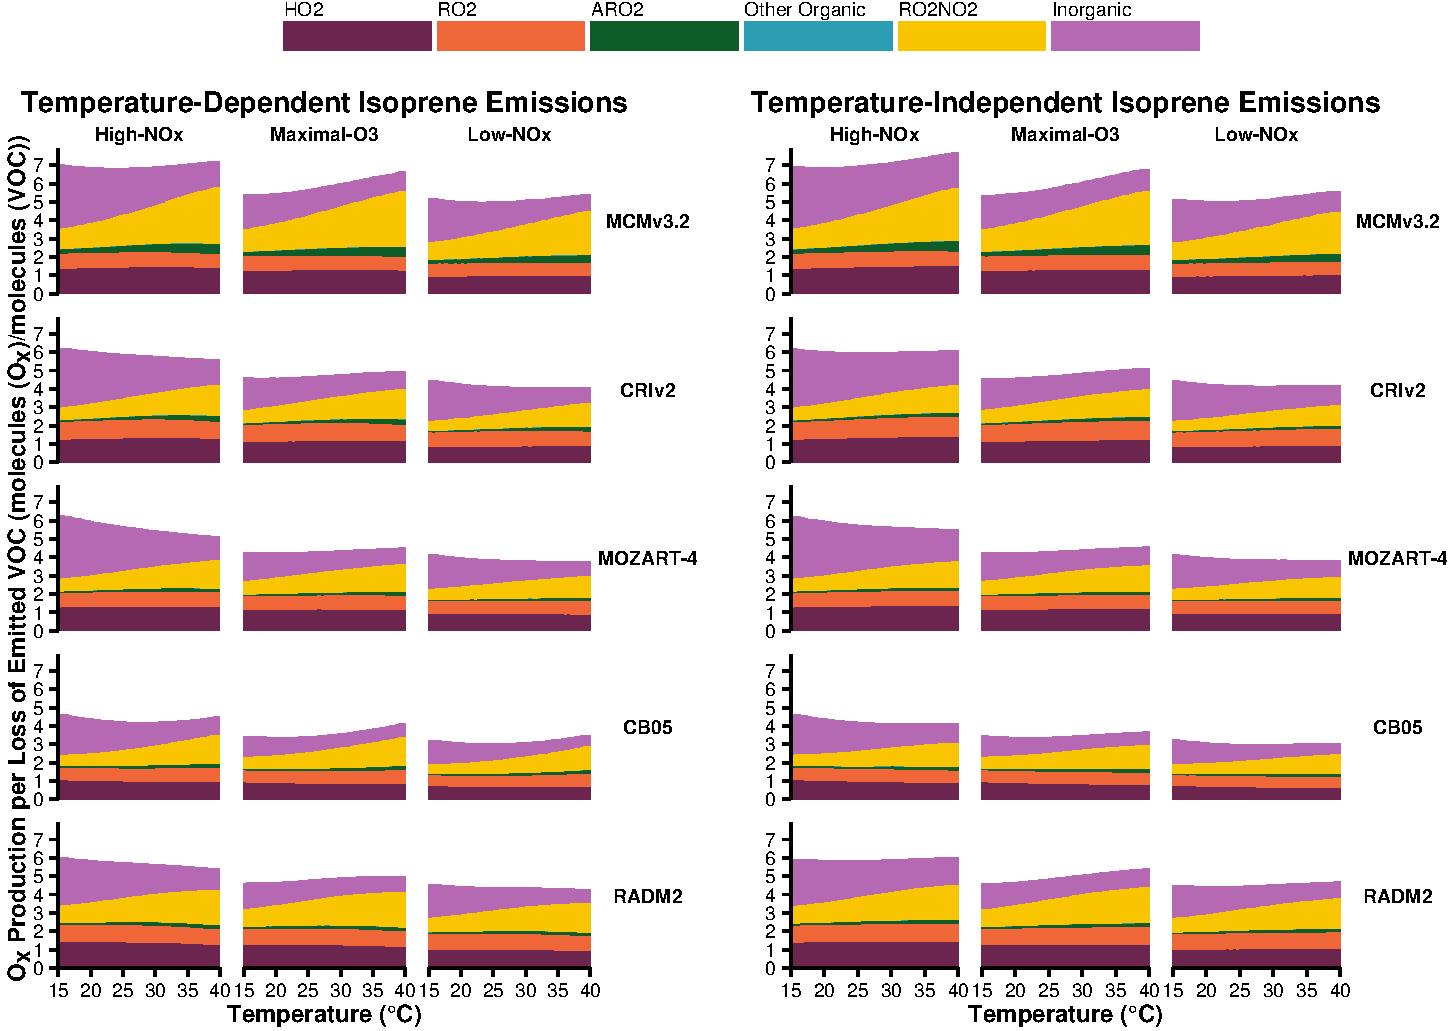
\includegraphics[width=\textwidth]{img/Ox_budgets}
\end{figure}

We defined the \ce{O_x} family to consist of \todo{complete this and reasons}

\citet{Sillman:1995} shows that the ratio of \ce{HNO3} to \ce{H2O2} can be used to determine whether an atmospheric system is in a \ce{NO_x}-sensitive, VOC-sensitive or in the ridge region of the \ce{NO_x}-VOC relationship with ozone, where maximum ozone is produced.
Based on this, we assigned each model run used to generate the ozone contours in Fig.~\ref{f:ozone_contours} to three \ce{NO_x} regimes--Low-NOx, High-NOx and Maximal-O3--corresponding to \ce{NO_x}-sensitive, VOC-sensitive and \ce{NO_x}-VOC-sensitive regions defined by \citet{Sillman:1995}.
Values of \ce{H2O2}/\ce{HNO3} less than $0.3$ correspond to the High-NOx regime, values larger than $0.5$ correspond to the Low-NOx regime and all values inbetween correspond to the ridge area in which maximal ozone is produced.

In Fig.~\ref{f:ozone_budgets}, the production rates on the first day of each reaction contributing to the \ce{O_x} production budget are determined and these reaction rates are then averaged over each \ce{NO_x}-condition (Low-\ce{NO_x}, High-\ce{NO_x} and Maximal-O3).
The fractional contribution of this reaction rate to the total \ce{O_x} budget was then calculated for each \ce{NO_x}-condition.

Figure~\ref{f:ozone_budgets} shows that the reaction of the hydroperoxyl radical (\ce{HO2}) with NO has the largest contribution at each \ce{NO_x}-condition, but this fractional contribution decreaes at higher temperatures due to the increased contributions of other reactions.
The increased contribution of the reaction of the acetyl peroxy radical (\ce{CH3CO3}) with NO with temperature has the most significant contribution to the total \ce{O_x} budget and this contribution is higher in CB05 and RADM2 compared to the other chemical mechanisms.

Add quantitative values of differences.

%\subsection{Rate of Change of Ozone with Temperature} \label{ss:r_mO3-T}
%
%\begin{figure}%
%    \centering%
%    \caption{Correlation of mean ozone mixing ratio with temperature in Low-NOx, maximal-O3 and High-NOx conditions for each chemical mechanism. A linear relationship between mean ozone mixing ratios and temperature is inferred, regression statistics are found in Table~\ref{t:O3_T_stats}.}%
%    \label{f:rate_O3_T}%
%    %\includegraphics[width=\textwidth]{img/Mean_O3_T_NOx_conditions}
%\end{figure}
%
%\begin{table}%
%    \centering%
%    \caption{Regression statistics for the linear relationship between ozone mixing ratios and temperature shown in Figure~\ref{f:rate_O3_T}.}%
%    \label{t:O3_T_stats}%
%    \scalebox{.78}[.78]{{\renewcommand{\arraystretch}{1.2}
\begin{tabular}{c|c|cc|cc|cc}
	\hline\hline
    \multirow{2}{*}{\textbf{Mechanism}} & \multirow{2}{*}{\textbf{Isoprene Emissions}} & \multicolumn{2}{c|}{\textbf{Low-\chem{NO_x}}} & \multicolumn{2}{c}{\textbf{Maximal-\chem{O_3}}} & \multicolumn{2}{|c}{\textbf{High-\chem{NO_x}}} \\
    & & \textbf{Mixing} & \textbf{No Mixing} & \textbf{Mixing} & \textbf{No Mixing} & \textbf{Mixing} & \textbf{No Mixing} \\
	\hline\hline
	\multirow{2}{*}{MCMv3.2} & Temperature Independent & 0.28 & 1.01 & 0.51 & 1.36 & 0.59 & 0.96 \\ 
    & Temperature Dependent & 0.42 & 1.48 & 0.74 & 2.16 & 0.93 & 2.63 \\ 
	\hline
	\multirow{2}{*}{CRIv2} & Temperature Independent & 0.25 & 0.93 & 0.47 & 1.27 & 0.55 & 0.88 \\ 
    & Temperature Dependent & 0.40 & 1.44 & 0.71 & 2.09 & 0.90 & 2.52 \\ 
	\hline
	\multirow{2}{*}{MOZART-4} & Temperature Independent & 0.25 & 0.97 & 0.44 & 1.21 & 0.49 & 0.59 \\ 
    & Temperature Dependent & 0.38 & 1.43 & 0.65 & 1.98 & 0.81 & 2.05 \\ 
	\hline
	\multirow{2}{*}{CB05} & Temperature Independent & 0.39 & 1.30 & 0.67 & 1.72 & 0.79 & 1.45 \\ 
    & Temperature Dependent & 0.52 & 1.72 & 0.89 & 2.44 & 1.12 & 2.94 \\ 
	\hline
	\multirow{2}{*}{RADM2} & Temperature Independent & 0.37 & 1.31 & 0.61 & 1.64 & 0.70 & 1.28 \\ 
    & Temperature Dependent & 0.48 & 1.68 & 0.79 & 2.22 & 0.97 & 2.49 \\ 
	\hline\hline
\end{tabular}}}

%\end{table}
%
%Each model run was allocated the three \ce{NO_x}-conditions as described in Sect.~\ref{ss:r_budgets} and then the mean ozone mixing ratio in these \ce{NO_x} regimes were then correlated with temperature as shown in Fig.~\ref{f:rate_O3_T}.
%In literature, a linear relationship is typically reported between ozone and temperature and so the linear regression statistics are reported in Table~\ref{t:O3_T_stats}.
%
%The linear increase of ozone with temperature, m$_{\text{O3-T}}$ in Table~\ref{t:O3_T_stats}, is highest at high-NOx conditions for each chemical mechanism and for each temperature case of isoprene emissions.
%The high-NOx regime corresponds to the top regions of the contour plots in Fig.~\ref{f:ozone_contours} where increases in temperature would shift the ozone production towards the ridge of maximal ozone production, thus this increase in m$_{\text{O3-T}}$ is expected.
%Similarly, the lowest m$_{\text{O3-T}}$ are achieved in the low-NOx regime, the bottom regions of the contours in Fig.~\ref{f:ozone_contours}, where increases in temperature do not neccisarily lead to increased ozone levels.
